\chapter{Concept}
This chapter will cover identified problems that occur when using AMCS via a web browser on mobile
devices. To narrow down the extend of this work, the system is analyzed from the point of view that an audience member like a student has while using AMCS on their smartphone. When doing so, students will interact mostly with the Main View and the Navigation, which are the components that this work will focus on.

\section{Problems of the mobile view}

The web page of AMCS reacts on requests coming from mobile devices such as smartphones or tablets by providing a responsive mobile view to its clients. However, in some aspects AMCS struggles to offer a UI experience that guarantees high usability and uniformity across all end user devices.
One challenge lays in the fact that the system has to deal with limited screen space to visualize information as effectively as possible. Additionally, users might approach the application with different ways of interaction and navigation in mind that are typical for mobile devices. For example, a smartphone user might expect to be able to use swiping gestures to navigate a menu or that information is organized in views consisting of separate tabs. This section lists key issues that lower usability or might cause confusion to users when using the system on a smartphone.

\subsection{Main View}
As already described in section \todosct, the main view relies on a vertically scrolling list view, consisting of different sections. The layout in place causes problems regarding usability aspects of the application.

\subsubsection{General Visualization Problems}
\label{section:con:problems:mainview:generalvis}
Section \todosct covered the fact, that lectures are rendered by displaying the title of the lecture in the top section of the box in white letters on a solid blue background. It is followed by detail information about the lecture such as time, duration and a textual description, visualized in grey letters and icons in a white screen. Finally, at the bottom of the box, the course name is shown in gray letters on a light blue background. The order "lecture name then details and then course name" can cause confusion to students.

The most coarse grain piece of information - the course name - is displayed at the bottom of the box rather than at the top. Generally, when seeking information about active lectures, a student will most likely remember the course name rather than the name of a single lecture, as timetables used by students only contain course names.
They will start to scan the displayed information with their eyeballs from top to bottom. Therefore, displaying the course information out of order might cause confusion and students take longer time to find the pieces of information that they are looking for.
In addition to that, no iconography or colors are used to differentiate between course name and lecture name.

\subsubsection{Indirection Problems}

The boxes that represent each lecture claim a lot of screen space in relation to the information that is displayed to the student. The layout causes a lot of indirection, because per default, the sections for upcoming and active lectures are expanded fully. This might be handy when quickly gathering information about lectures that are or soon will be active, but in every other case it slows navigation and overall interaction, because the course management section is pushed down to the bottom of the page.
A list of only four boxes causes a scroll bar to appear on the very common screen resolution of 1920x1080 pixels. A student that navigates to the main view to enroll into a new course therefore always has to scroll to the bottom of the page before they reach the enrollment form. The same problem likewise occurs when simply seeking information about what courses a student is already enrolled in or when trying to leave a course altogether. 

Further more, if a student looks for information regarding a specific course, no filter or search functionality is offered by the lecture list. Instead, they have to scroll down to the bottom of the lecture list, scan the course list manually with their eyeballs, find the course and click on the corresponding item. Finally, they are redirected to the course view. This level of indirection is only further increased the more courses the student is enrolled in. 
To sum it up, the hierarchical and logical relationship between courses and lectures is broken. 

\subsubsection{Redundancy}

Some visual redundancy is added by the badges that are displayed on the top right corner of each lecture. These badges are used to visualize the temporal context of the lecture for each item in the corresponding section. It seems that the badge's intention is to help conveying the temporal context of the lecture, because sorting the lectures in their respective section alone fails to do so. Furthermore, the badge's names do not match the section's names, e.g. an upcoming lecture's badge reads “BEFORE” instead of “UPCOMING”. 

In the course management section below, for each course the student is enrolled in, a box is shown with the course's name along with an unsubscribe button, represented by a trash can icon.
\todogrf
This is a redundant way of rendering the courses which adds noise to the overall look of the view and uses much of the vertical screen estate.

\subsection{Course View}
\todo{Add this}

Since the course view reuses the lecture list along with the sections “Upcoming lectures”, “Active lectures” and “Past lectures”, likewise the same issues arise as for the main view, as already described in section \ref{section:con:problems:mainview:generalvis}. 
The course view has a very important function in terms of usability as it acts as a filter for lectures belonging to a certain course. 

\todogrf

\subsection{Poll View}

\subsubsection{Rendering}

Section \todosct describes the rendering of questions as boxes that are aligned in a vertical scrolling list. This introduces similar problems as already described in section 3.1, namely the extensive use of vertical space on the screen. Bigger polls that consist of multiple questions unnecessarily take a lot of vertical screen estate. The view also lacks of basic information such as number of questions in total or number of remaining questions that might be useful in bigger polls if students want to gain an overview of how many questions are left.
Answering one question usually does not require to see the neighboring questions, but most of the time, two to three questions are in view simultaneously. This might be distracting to some students.
\todo{Provide screenshots and explain this better.}
Additionally, the layout lacks of separation and distinction between types of polls.
Different types of polls are simply appended to the bottom of the list, making it even longer.

\subsubsection{Local navigation}

The vertical list is difficult to navigate as it requires scrolling between questions. If a student wants to jump from the first to the last question,  or vice versa, several swiping gestures are needed to reach the top or the bottom of the list.
Similar to the lecture list described in \todosct, the question list is also segmented into different sections. Lecture and course questions are similarly appended to the bottom of a slide poll. This means again, that a student that wants to view these questions has to scroll all the way to the bottom of the list. Again, this layout introduces a lot of indirection and is not intuitive to the user.


\subsection{Burger Menu and Navigation}

At the time of writing, the ways of navigating the application can be described as problematic and partly confusing. Several layers of indirection introduce problems and may worsen the user experience.
The burger menu icon is located in the top right part of the header and offers most of the navigation functionality. Students have to tap on this icon to access menu that consists of sub menus as described in \todosct. 
One problem that arises is the fact that the menu uses a lot of vertical screen space and delocates the rest of the content that is currently shown.
In addition, the menu can be confusing to the student because the first entry is labeled as \emph{Student}. This implies to users in general that there exist different roles that a user can take on in AMCS, which is the case. But the user's role should not be the label of a sub menu in the navigation as it is not intuitive that functionality like account management can be accessed via a button labeled \emph{Student}.

\subsubsection{Evaluation of answers}

Clicking on the option “Evaluation of answers” button in the expanded burger menu leads to a view with a drop down menu from which students can choose a course that they are interested in. Afterwards, an list of expandable items is shown, where each item represents a lecture. Clicking on one or multiple of these items will expand a vertical list of questions similar to  the regular question list described in section \todosct, but answers given by the student are shown as well (see Fig. \todosct).
Multiple problems occur on this view: First of all, the navigation path to reach this view contains unnecessary indirection and might not be intuitive enough. Students might expect this functionality to be located at the main view attached to the elements of the course list or inside the course view itself. Instead, every time evaluation of given answers is attempted, this functionality can only be accessed by using the burger menu, choosing the appropriate item from the sub menu, selecting the course in question and afterwards expand the lecture and the corresponding question list.
\todo{Insert a graphic that visualizes the click path that is problematic}
Additionally, the question list suffers from the same rendering and navigation problems already described in \todosct. Questions are poorly navigable and a lot of scrolling is needed to jump between questions.



\begin{figure}[ht]
	\centering
	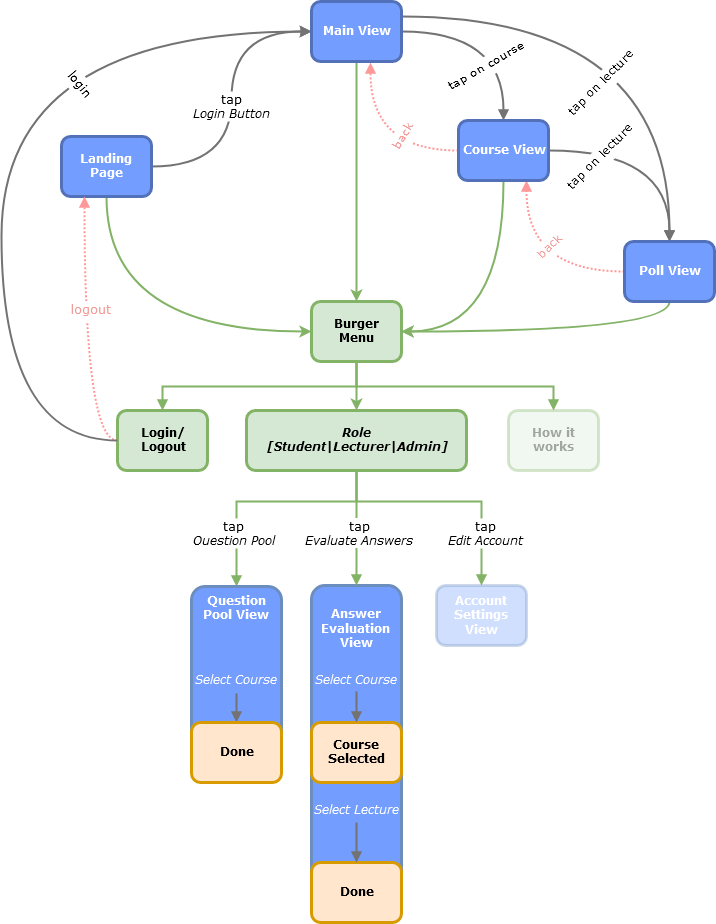
\includegraphics[width=\textwidth]{diagrams/amcs-click-paths.png}
	\caption{um 30 Grad gedreht}
	\label{fig1}
\end{figure}
\subsubsection{Question Pool}

The question pool suffers from the same navigation problems described in the previous section. Again, a drop down menu for selecting a course is shown before students can see the overview of the question pool. Once more, students might think that access to this functionality is located near the main view or the course view, which is not the case.

\todo{Add a table that names and describes all analyzed weaknesses so that the proposals chapter can refer to this}

